\section{Contexto del proyecto}

\subsection{Modelo de Ciclo de Vida}

La naturaleza del proyecto determina cuál metodología se elige antes de analizar las alternativas. Cuando el aporte de un trabajo investigativo no es una teoría ni la observación de algún fenómeno, sino la construcción de un sistema que resuelve un problema real, la metodología más acorde al Kit Pagos Colombia es Design Science Research (DSR) (Peffers, K., Tuunanen, T., Rothenberger, M., \& Chatterjee, S, 2007). Esta metodología organiza el proceso alrededor de una pregunta central: ¿el artefacto fue construido correctamente y resuelve el problema para el que fue diseñado? Esas dos dimensiones, estructuran las fases del proyecto y le dan coherencia a la investigación.

% El original no tiene 3.1.1, y el texto cita la 3.1.3 en las secciones 5.2.1, 6, 7.1 y 7.4.
\setcounter{subsubsection}{1}
\subsubsection{Adaptación del ciclo de vida}

\begin{itemize}
  \item \textbf{Identificación y definición del problema:} Consiste en estudiar las documentaciones técnicas de Wompi, Rapyd (que adquirió PayU GPO), Mercado Pago y Kushki para identificar sus diferencias en aspectos relevantes para su implementación tales como, autenticación, estructuras de respuesta, manejo de webhooks y comportamiento ante errores. El resultado de esta fase es una especificación técnica que traduce la fragmentación del ecosistema en requerimientos funcionales concretos para el framework. Esta fase produce el mapa del ecosistema y el repositorio de parámetros de prueba.
  \item \textbf{Definición de objetivos:} A partir del análisis anterior se delimita el alcance del framework: qué operaciones debe soportar, bajo qué criterios se seleccionaron las pasarelas, cómo se medirá el éxito del proyecto y cuales son las características que deben tener los proyectos prototípicos usados en la evaluación. Esta fase produce el documento de alcance, los criterios de evaluación formalizados y el backlog inicial.
  \item \textbf{Diseño:} Aquí las decisiones del documento de alcance se convierten en contratos arquitectónicos verificables: el modelo de dominio unificado del framework, los puertos de la arquitectura hexagonal, la especificación de los adaptadores por cada pasarela y el diseño de la API de simulación con sus escenarios de prueba. Esta fase produce un conjunto de artefactos de diseño que orientan el desarrollo sin ambigüedad y que también funcionan como criterios de corrección durante la implementación.
  \item \textbf{Desarrollo:} Es la fase más extensa del proyecto y la única que opera de forma iterativa internamente. Se construye en tres iteraciones dependientes:
  \begin{itemize}
    \item El núcleo del framework con sus contratos de puerto.
    \item Los adaptadores de cada pasarela con bajo acoplamiento, siendo independientes entre sí.
    \item La API de Simulación completa, la documentación de datos de prueba, la página de presentación y los prototipos B y D, los cuatro entregables que \texttt{methodology.md} (sección 2.1) asigna a esta iteración.
  \end{itemize}
  El orden no es arbitrario: la arquitectura hexagonal impone que el núcleo y sus contratos existan antes de que cualquier adaptador pueda construirse correctamente. La versión 1.0 de este plan ponía los prototipos en la fase de demostración; sus issues (\#150 y \#151) quedaron en el hito de la Iteración 3 y se cerraron el 25 de octubre de 2026.
  \item \textbf{Demostración y evaluación:} El framework se aplica en los proyectos prototípicos y sobre el código resultante se miden seis variables, entre ellas las métricas WMC, CBO y RFC de Chidamber y Kemerer (1994). El prototipo B, que usa el framework, se compara con el D, que integra las cuatro pasarelas directamente contra sus APIs nativas, lo que constituye el núcleo experimental del proyecto (\path{docs/project-management/prototypes-evaluation-plan.md}). En paralelo de esta evaluación, sucede la demostración, siendo esta el acto de integrar el framework en los prototipos.
  \item \textbf{Comunicación:} Esta fase comprende la consolidación del documento de trabajo de grado y la publicación del repositorio público con documentación suficiente para que un desarrollador externo pueda integrar el kit sin haber estado involucrado en el desarrollo del mismo. Aunque esta fase cierra formalmente el ciclo DSR, su redacción comienza desde las primeras fases: el documento de grado no es una actividad de cierre sino un artefacto que crece en paralelo con el proyecto.
\end{itemize}

\subsubsection{Hitos del ciclo de vida}

Los seis hitos que marcan el avance del ciclo de vida son:

\begin{itemize}
  \item H1: el mapa del ecosistema completo y el repositorio de parámetros de prueba validado.
  \item H2: la arquitectura del framework diseñada con contratos de puerto especificados.
  \item H3: el núcleo del SDK funcional con al menos un adaptador operativo.
  \item H4: los cuatro adaptadores y la API de simulación completos y con pruebas internas aprobadas; H5, los proyectos prototípicos evaluados con las métricas CK (Chidamber, Kemerer, 1994) registradas; y H6, el repositorio público publicado y el documento de grado entregado.
\end{itemize}

La Tabla~\ref{tab:hitos-reales} compara la semana en que el plan ubicaba cada hito con la fecha en que se alcanzó. Las semanas S01 a S18 de la versión 1.0 no tenían fechas; aquí se anclan al calendario con la Iteración 1 en la semana del 24 de agosto de 2026, como hace \texttt{methodology.md} (sección 10.2), así que la S01 empieza el 13 de julio. Las fechas reales salen del último issue cerrado de cada hito de GitHub, en hora de Colombia, y de las respuestas del equipo para las Fases 1 y 2.

\begin{center}
\renewcommand{\arraystretch}{1.2}
\begin{longtable}{|P{0.12}|P{0.22}|P{0.28}|P{0.38}|}
  \hline
  \textbf{Hito} & \textbf{Plan (versión 1.0)} & \textbf{Real} & \textbf{Fuente} \\
  \hline
  \endfirsthead
  \hline
  \textbf{Hito} & \textbf{Plan (versión 1.0)} & \textbf{Real} & \textbf{Fuente} \\
  \hline
  \endhead
  \caption{Fechas planeadas y reales de los hitos.}
  \label{tab:hitos-reales}\\
  \endlastfoot
  H1 & S03 (hasta el 2 de agosto) & Junio de 2026 & Las Fases 1 y 2 se hicieron entre abril y junio de 2026, según el equipo. Los datos de prueba se validaron después, con mediciones fechadas desde el 18 de septiembre (\texttt{docs/testing-data/README.md}, sección 3) \\
  \hline
  H2 & S07 (hasta el 30 de agosto) & 6 de septiembre de 2026 & Último cierre del hito «Fase 3 – Diseño (cierre)» \\
  \hline
  H3 parcial & S08 (hasta el 6 de septiembre) & 15 de septiembre de 2026 & Último cierre de la Iteración 1 \\
  \hline
  H3 completo & S10 (hasta el 20 de septiembre) & 21 de septiembre de 2026 & Último cierre de la Iteración 2 \\
  \hline
  H4 & S12 (hasta el 4 de octubre) & 9 de noviembre de 2026 & Último cierre de la Iteración 3 (\#112, la documentación oficial del producto) \\
  \hline
  H5 & S16 (hasta el 1 de noviembre) & 9 de noviembre de 2026 & Último cierre de la Fase 5 (\#135): el informe comparativo (\path{docs/evaluation/informe-comparativo-fase-5.md}), sobre las seis variables medidas el 22 y el 28 de octubre \\
  \hline
  H6 & S18 (hasta el 15 de noviembre) & Entrega prevista el 9 de noviembre de 2026 & Hito «Fase 6 – Comunicación» \\
  \hline
\end{longtable}
\end{center}

La Figura~\ref{fig:ciclo-de-vida} ilustra el ciclo de vida del proyecto. La fase 4 al ser el desarrollo se tomará como iterativa de manera interna a la misma con el fin de garantizar un desarrollo ágil.

\begin{figure}[H]
  \centering
  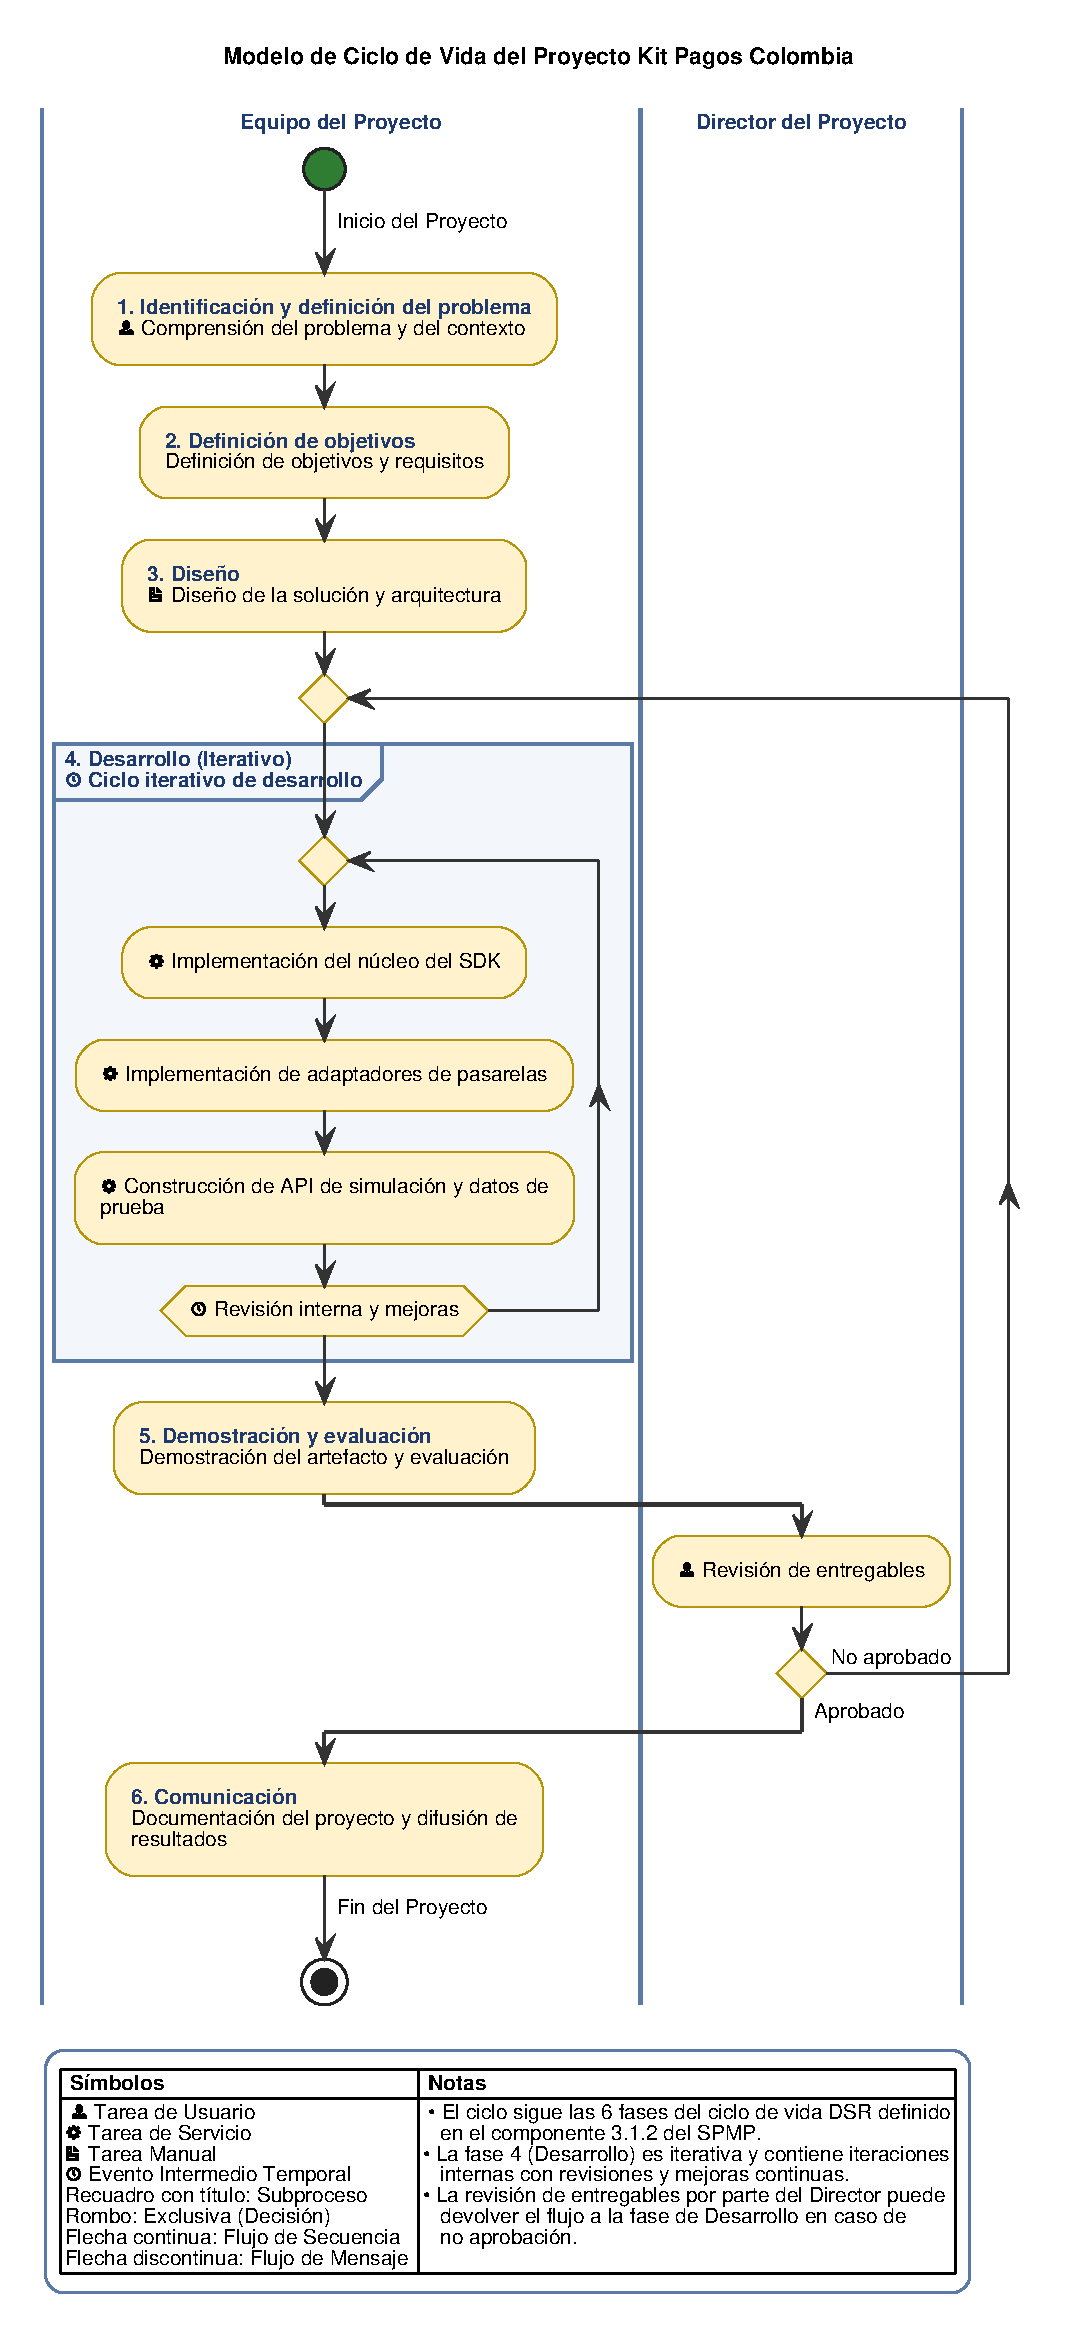
\includegraphics[width=\textwidth,height=0.93\textheight,keepaspectratio]{figuras/01-ciclo-de-vida}
  \caption{Adaptación del Ciclo de Vida.}
  \label{fig:ciclo-de-vida}
\end{figure}

\subsubsection{Análisis de Alternativas y Justificación}

Antes de justificar la elección de DSR, es necesario revisar los modelos que se consideraron y por qué no resultan suficientes para este proyecto.

\textbf{Modelo en cascada}

El modelo en cascada estructura el desarrollo en fases secuenciales: análisis de requisitos, diseño, implementación, pruebas y despliegue, con transiciones unidireccionales entre ellas. Su mayor fortaleza es la claridad estructural que ofrece, lo que facilita la planificación anticipada y la documentación sistemática. Sin embargo, su rigidez resulta problemática para proyectos en los que el entendimiento del problema evoluciona a medida que se trabaja en él.

En el caso del Kit Pagos Colombia, la fase de análisis de las APIs consiste en estudiar cuatro documentaciones técnicas distintas, y es habitual que ese proceso revele detalles que afecten las decisiones de diseño. El modelo en cascada no tiene mecanismos formales para incorporar esos hallazgos una vez que la fase de análisis ha cerrado. Adicionalmente, la dimensión investigativa del proyecto (evaluar el artefacto y compararlo con un enfoque alternativo) no tiene lugar natural dentro del ciclo cascada, que asume que el sistema se entrega y eso constituye el fin del proceso.

\textbf{Modelo incremental}

El modelo incremental mejora la adaptabilidad del cascada al proponer la entrega del sistema en partes funcionales progresivas. Cada incremento produce una versión del sistema que puede ser evaluada antes de proceder al siguiente. Esto es especialmente útil cuando los requisitos no están completamente definidos desde el inicio.

Sin embargo, el modelo incremental no proporciona un marco metodológico para la generación de conocimiento académico ni para la validación científica de artefactos. En este proyecto, la evaluación no es simplemente "funciona o no funciona": es una comparación cuantitativa entre dos enfoques de integración usando métricas de ingeniería de software, lo que requiere un diseño experimental explícito. El modelo incremental no contempla ese componente. Adicionalmente, la arquitectura hexagonal impone un orden de construcción específico (núcleo antes que adaptadores) que no corresponde necesariamente al orden de valor de negocio que guía un incremento típico.

\textbf{Scrum}

Scrum es el marco de trabajo ágil más extendido. Organiza el desarrollo en sprints cortos con retrospectivas, backlog priorizado y participación activa de un Product Owner que representa las necesidades del usuario final. Sus fortalezas en adaptabilidad y entrega continua de valor son bien conocidas.

El problema de aplicar Scrum como marco principal en este proyecto es doble. Por un lado, no hay un cliente externo: el Product Owner sería en la práctica el equipo mismo, lo que elimina el mecanismo de validación externa que Scrum presupone. Por otro lado, Scrum tampoco ofrece un marco para la contribución académica ni para la evaluación sistemática del artefacto contra un escenario de control. Un proyecto de grado no puede limitarse a entregar software funcional; debe justificar por qué ese software resuelve el problema mejor que las alternativas existentes, y para eso necesita un método.

Esto no significa que Scrum sea irrelevante para el proyecto. Dentro de la fase de desarrollo de DSR, los principios de Scrum son útiles para organizar el trabajo iterativo: el backlog permite priorizar componentes, los sprints cortos (de una semana) ayudan a mantener el ritmo, y las revisiones periódicas facilitan la detección temprana de problemas de implementación. Scrum se incorpora entonces como práctica interna de la fase 4, no como marco metodológico del proyecto completo.

\textbf{Design Science Research (DSR)}

DSR fue propuesto por Peffers et al. (2007) como metodología para proyectos cuyo resultado central es la construcción de un artefacto que resuelve un problema real. A diferencia de los modelos anteriores, DSR integra explícitamente la investigación y la construcción: no basta con que el sistema funcione, debe evaluarse su efectividad frente al problema que motivó su creación y los resultados deben comunicarse de forma rigurosa.

Las seis fases adaptadas de DSR corresponden directamente a lo que este proyecto necesita hacer: identificar y caracterizar el problema de la fragmentación de las APIs colombianas de pago; definir los objetivos del framework y los criterios con que se medirá su éxito; diseñar la arquitectura del SDK y la API de simulación; construir el artefacto; demostrarlo y evaluarlo con las métricas CK; y comunicar los resultados a través del documento de grado y el repositorio público.

Ninguno de los modelos anteriores ofrece ese recorrido completo. DSR es la única metodología que exige los tres elementos que este proyecto requiere: rigor en el diseño del artefacto, un mecanismo de evaluación experimental y un componente de comunicación académica.

\textbf{Prácticas específicas adoptadas}

El modelo de ciclo de vida no se ejecuta de forma monolítica. Para los aspectos más importantes del proyecto se adoptan prácticas específicas que complementan DSR.

Para la fase de análisis de APIs, se utiliza revisión documental estructurada: cada integrante estudia la documentación oficial de una o dos pasarelas y produce un mapa de diferencias técnicas que luego se consolida en equipo. Esto garantiza que el análisis sea sistemático y que los hallazgos queden documentados de forma trazable.

Para las decisiones de diseño arquitectónico, se usan documentos breves que registran qué decisión se tomó, qué alternativas se consideraron y por qué se eligió la opción seleccionada. Esto es especialmente útil para decisiones sobre la estructura de los puertos del SDK y las convenciones de normalización de respuestas, que no siempre son obvias y tienden a revisitarse durante el desarrollo.

Para el desarrollo de los adaptadores, que son el componente de mayor complejidad técnica, se aplica programación en pares. Dos integrantes trabajan juntos en cada adaptador, reduciendo la probabilidad de errores y distribuyendo el conocimiento específico de cada pasarela dentro del equipo. El núcleo del SDK, por su naturaleza más conceptual y por ser la base sobre la que depende todo lo demás, es revisado por todos los integrantes antes de que comience la implementación de los adaptadores.

Para las pruebas, el framework se valida primero contra la API de simulación propia antes de validarse contra los sandboxes reales de las pasarelas. Esto reduce la dependencia de credenciales externas durante el desarrollo y permite pruebas más controladas y reproducibles. Las pruebas unitarias sobre el núcleo y las pruebas de integración sobre los adaptadores se automatizan desde el principio y se ejecutan en cada pull request mediante integración continua.

Para la revisión de código, se adopta una política estricta de pull requests: ningún cambio entra a las ramas \texttt{devops} y \texttt{main} sin un pull request revisado por al menos otro integrante (\texttt{CONTRIBUTING.md}). Esto funciona como mecanismo de control de calidad continuo y también como transferencia de conocimiento entre quienes trabajan en frentes distintos del framework.

Para la evaluación con métricas CK, el diseño experimental se fija antes de medir y no se improvisa al llegar a la fase 5. Los proyectos prototípicos y la herramienta de medición se definen con anticipación, igual que las unidades sobre las que se calculan las métricas: archivos, desde el issue \#134 (\texttt{methodology.md}, sección 6.1.1). Así, la comparación entre integración directa e integración con el framework es reproducible y no queda sujeta a sesgos de selección posterior.
